%-----------------
% verso e anverso:
%-----------------
%\documentclass[10pt,twoside,openany,a4paper,portuguese]{abntex2}	
\documentclass[
% -- opções da classe memoir --
12pt,				 % tamanho da fonte
openright,           % capítulos começam em pág ímpar (insere página vazia caso preciso)
oneside,			 % impressão somente em um lado da folha. [ twoside | oneside]
a4paper,			 % tamanho do papel. 
sumario=tradicional, %% formato do sumário
% -- opções da classe abntex2 --
chapter=TITLE,		 % títulos de capítulos convertidos em letras maiúsculas
%	section=TITLE,		 % títulos de seções convertidos em letras maiúsculas
%	subsection=TITLE,	 % títulos de subseções convertidos em letras maiúsculas
%	subsubsection=TITLE, % títulos de subsubseções convertidos em letras maiúsculas
% -- opções do pacote babel --
fleqn,				 % Alinha equações numeradas pela esquerda.
english,
spanish,
brazil,				 % o último idioma é o principal do documento		
]{abntex2}%{/TexStudio/Modelos/unimontes-ppgmsc-abntex2}
% -------
% PACOTES
% -------

% --------------------
% Pacotes fundamentais 
% --------------------
\usepackage{graphicx}
\usepackage[export]{adjustbox}
\usepackage{cmap}				% Mapear caracteres especiais no PDF
\usepackage{mathptmx}
\usepackage{pslatex}		    % {pslatex} Usa a fonte Times New Romam
\usepackage{geometry}
\usepackage[utf8]{inputenc}		% Codificacao do documento (conversão automática dos acentos)
\usepackage[T1]{fontenc}		% Selecao de codigos de fonte.
\usepackage{tikz,fullpage}
\usepackage{indentfirst}		% Indenta o primeiro parágrafo de cada seção.
\usepackage{lscape}				% Mudar a orientação da página
\usepackage{color}				% Controle das cores
\usepackage[]{graphics}			% Inclusão de gráficos
\usepackage{xcolor}
\usepackage{listings}           % Inclusão de arquivos de código de programação
\usepackage{showexpl}           % exibe codigos de figuras
\usepackage{verbatim}           % incluir arquivos não processados pelo Latex
\usepackage{colortbl}			% Permitir colorir células na tabela
\usepackage{placeins}			%

\usepackage{amsmath}			%
\usepackage{amssymb}			%
\usepackage{tabto}				%
\usepackage{longtable}			% Permitir tabelas maiores que o comprimento da página, quebra automática
\usepackage{booktabs}
\usepackage{array}
\usepackage{float, caption}		% Incluir novos rotulos a figura http://ctan.org/pkg/float
\usepackage{tocbasic}			% Criar novas listas de Mapas, Photos e Figuras
\usepackage{tocloft, xparse}	% Criar a lista de gráficos
\usepackage{titlesec}
%\usepackage{algorithm} %
\usepackage{tocbibind}
\usepackage[portuguese,ruled,lined,vlined]{algorithm2e} % Inclusão de algoritmos(pseudo código) em portugues
\usepackage{etoolbox}			% http://ctan.org/pkg/etoolbox
\usepackage{microtype} 			% para melhorias de justificação
\usepackage{pgf}
\usepackage{pdfpages}			% incluir arquivos pdf no texto
\usepackage{multirow}
\usepackage{tabularx}
\usepackage{bigstrut}
\usepackage[utf8]{inputenc}


\usetikzlibrary{arrows,automata}

%-\---------------


% -------------------
% Pacotes de citações
% -------------------
%\usepackage[brazilian,hyperpageref]{backref}	 % Paginas com as citações na bibl
\usepackage[alf, abnt-etal-cite=1]{abntex2cite} %\usepackage[alf]{abntex2cite}	% Citações padrão ABNT

%---------------------
% Definindo o tamanho e aparência dos títulos do trabalho
%---------------------
\renewcommand{\tocheadstart}{\ABNTEXchapterfont}
\renewcommand{\ABNTEXchapterfont}{\fontfamily{ptm}\fontseries{b}\selectfont}
\renewcommand{\ABNTEXchapterfontsize}{\Large}

%\titleformat{\Comando de Estructura}[Tipo]{Formato}{Etiqueta}{Separación}{Código anterior}[Código posterior]
\titleformat{\chapter}[hang]{\normalfont\Large\bfseries}{\thechapter}{12pt}{\Large}

\makeatletter
% Formatação do capítulo \chapter para exibição na página onde foi definido
\def\@makechapterhead#1{%
	\begin{center}
		\reset@font{\ABNTEXchapterfont\Large\noindent\textbf{\thechapter~\texorpdfstring{#1}{#1}}} \par%		
	\end{center}
	\vspace{18pt}
}

\makeatother

%----------------------------------------
% Definição de cores utilizadas no código
%----------------------------------------
\definecolor{dkgreen}{RGB}{0,0.6,0}
\definecolor{gray}{RGB}{0.5,0.5,0.5}
\definecolor{mauve}{RGB}{0.58,0,0.82}
\definecolor{verde}{RGB}{0.25,0.5,0.35}
\definecolor{verdecpp}{RGB}{0,0.5,0}
\definecolor{verdejava}{RGB}{0.25,0.5,0.35}
\definecolor{jpurple}{RGB}{0.5,0,0.35}
\definecolor{mygreen}{RGB}{0,0.6,0}
\definecolor{mygray}{RGB}{0.5,0.5,0.5}
\definecolor{mymauve}{RGB}{0.58,0,0.82}
\definecolor{blue}{RGB}{41,5,195}
\definecolor{graytb}{RGB}{0.8,0.8,0.8}
\definecolor{lightgray}{gray}{0.9}

%-----------------------------
% configuração de codigo fonte
%-----------------------------
\lstdefinestyle{Java}
{
	language={Java},
	inputencoding=,
	basicstyle=\ttfamily\small, 
	keywordstyle=\color{jpurple}\bfseries,
	stringstyle=\color{red},
	commentstyle=\color{verdejava},
	morecomment=[s][\color{blue}]{/*}{*/},
	morecomment=[l][\color{blue}]{//},
	extendedchars=true, 
	showspaces=false, 
	showstringspaces=false, 
	extendedchars=true, 
	numbers=left,
	numberstyle=\tiny,
	breaklines=true, 
	backgroundcolor=\color{cyan!10}, 
	breakautoindent=true, 
	captionpos=b,
	xleftmargin=0pt,
	tabsize=4
}

% -----------------------------------------------
% Informações de dados para CAPA e FOLHA DE ROSTO
% -----------------------------------------------
\titulo{Desenvolvimento de um aplicativo para coleta de informações geográficas voluntárias sobre problemas urbanos}
\autor{Liara Pereira Duarte}
\local{Almenara - MG}
\data{Janeiro - 2019}
\instituicao{Instituto Federal do Norte de Minas Gerais -- IFNMG \par Departamento do Trabalho \par Análise e Desenvolvimento de Sistemas} 
\tipotrabalho{TCC (Graduação)}

\preambulo{Documento apresentado a banca examinadora designada pelo Colegiado do Curso Análise e Desenvolvimento de Sistemas -- ADS, como parte dos requisitos necessários à obtenção do grau de Tecnólogo em Análise e Desenvolvimento de Sistemas.
\newline
\newline
Orientador: Prof. Alfredo Costa
} 


% ---



%-------------------
% informações do PDF
%-------------------
\makeatletter

\hypersetup{
	%pagebackref=true,
	pdftitle={\@title}, 
	pdfauthor={\@author},
	pdfsubject={\imprimirpreambulo},
	pdfcreator={nome do trabalho},
	pdfkeywords={palavras chave}{multiobjetivo}{Pareto local search}, 
	colorlinks=true,       		% false: boxed links; true: colored links
	linkcolor=black,          	% color of internal links
	citecolor=black,        	% color of links to bibliography
	filecolor=black,      		% color of file links
	urlcolor=black, 			% color of url links
	bookmarksdepth=4
}

%---------------------------------


%
%% Define os comandos que montam a lista de símbolos
\newcommand{\listadesimbolos}{\pretextualchapter{LISTA DE SÍMBOLOS}\@starttoc{lsb}}
\setuptoc{lgf}{chapteratlist}
\newcommand{\simbolo}[2]{{\addcontentsline{lsb}{simbolo}{\numberline{#1}{#2}}}#1}
\newcommand{\l@simbolo}[2]{
	\vspace{-0.75cm}\leftskip 0em 
	\parindent 0em \@tempdima 5em
	\advance\leftskip \@tempdima
	\null\nobreak\hskip -\leftskip
	{\normalfont #1}\hfil\nobreak\par}

% Define o comando que monta a lista de siglas
%\usepackage{nomencl}
%\makenomenclature
%\renewcommand{\nomname}{LISTA DE ABREVIATURAS E SIGLAS}
%
%\newcommand*{\sigla}[2]{#1\nomenclature{#1}{#2}}
\newcommand{\listadesiglas}{\pretextualchapter{LISTA DE ABREVIATURAS E SIGLAS}\@starttoc{lsg}}
\newcommand{\sigla}[2]{{\addcontentsline{lsg}{sigla}{\numberline{#1}{#2}}}#1}
\newcommand{\l@sigla}[2]{
	\vspace{-0.75cm}\leftskip 0em
	\parindent 0em \@tempdima 5em
	\advance\leftskip \@tempdima
	\null\nobreak\hskip -\leftskip
	{\normalfont #1}\hfil\nobreak\par}
\makeatother
% --- 

%---------------------------------------
% Criação do indice de gráficos
%---------------------------------------

\DeclareNewTOC[%
type=grafico,%
types=graficos,% used in the \listof.. command
float,% define a floating environment
floattype=4,% see below
name=Gráfico,%
listname={Lista de Gráficos}%
]{lgf}

%%% --- 

\DeclareNewTOC[%
type=quadro,%
types=quadros,% used in the \listof.. command
float,% define a floating environment
floattype=4,% see below
name=Quadro,%
listname={Lista de Quadros}%
]{loq}
\setuptoc{loq}{chapteratlist}

%%% --- 

\DeclareNewTOC[%
type=algoritmo,%
types=algoritmos,% used in the \listof.. command
float,% define a floating environment
floattype=4,% see below
name=Algoritmo,%
listname={Lista de Algoritmos}%
]{loa}
\setuptoc{loa}{chapteratlist}

%%% --- 


%-----------------------------------------
% Definindo o tamanho e alinhamento das colunas de uma tabela
%-----------------------------------------
\newcolumntype{L}[1]{>{\raggedright\let\newline\\\arraybackslash\hspace{0pt}}m{#1}}
\newcolumntype{C}[1]{>{\centering\let\newline\\\arraybackslash\hspace{0pt}}m{#1}}
\newcolumntype{R}[1]{>{\raggedleft\let\newline\\\arraybackslash\hspace{0pt}}m{#1}}

% --- 
% Espaçamentos entre linhas e parágrafos 
% --- 
\geometry{a4paper, left=3cm, right=2cm, bottom=2cm, top=3cm, headsep=1cm, footskip=2.2cm}
\setlength{\parindent}{2cm} 		% O Recuo de 1ª linha do parágrafo
\renewcommand{\baselinestretch}{1.5}	% espaçamento entre linhas 

% ----------------
% compila o indice
% ----------------
\makeindex
% ---


% -------------------
% Início do documento
% -------------------
\begin{document}


	% Retira espaço extra obsoleto entre as frases.
	\frenchspacing 
	
	%-------------------------------------------------------
	% Configurar a lista de gráficos
	%-------------------------------------------------------
	\newlistof{listofgraficos}{lgf}{\listofgraficosname}
	\newcommand{\listofgraficosname}{Lista de gráficos}
	\newlistentry{grafico}{lgf}{0}
	\renewcommand{\cftgraficoname}{\graficoname\space}
	\renewcommand*{\cftgraficoaftersnum}{\hfill\textendash\hfill}
	%----- ----- ----- ----- ----- ------ ----- ----- ----- ----- ----- ------ --
	
	%-------------------------------------------------------
	% Configurar a lista de quadros
	%-------------------------------------------------------
	\newlistof{listofquadros}{loq}{\listofquadrosname}
	\newcommand{\listofquadrosname}{Lista de quadros}
	\newlistentry{quadro}{loq}{0}
	\renewcommand{\cftquadroname}{\quadroname\space}
	\renewcommand*{\cftquadroaftersnum}{\hfill\textendash\hfill}
	%----- ----- ----- ----- ----- ------ ----- ----- ----- ----- ----- ------ --
	
	%%-------------------------------------------------------
	%% Configurar a lista de algoritmos
	%%-------------------------------------------------------
	\newlistof{listofalgoritmos}{loa}{\listofalgoritmosname}
	\newcommand{\listofalgoritmosname}{Lista de Algoritmos}
	\newlistentry{algorithm}{loa}{0}
	\renewcommand{\cftalgorithmname}{\algorithmname\space}
	\renewcommand*{\cftalgorithmaftersnum}{\hfill\textendash\hfill}
	%----- ----- ----- ----- ----- ------ ----- ----- ----- ----- ----- ------ --

% ----------------------------------------------------------
% ELEMENTOS PRÉ-TEXTUAIS
% ----------------------------------------------------------
\pretextual

% ----
% Capa
% ----
\imprimircapa
\clearpage
% ---

% --------------
% Folha de rosto
% --------------
\imprimirfolhaderosto
\clearpage
% ---
% ----------------------------------------------------------------------- %

% ---
% Dedicatória
% ---

% ---




% ---
% Agradecimentos
% ---
\begin{agradecimentos}
Em primeiro lugar a Deus, que sempre me deu forças para continuar mesmo quando pensei em desistir muitas vezes, em segundo lugar dedico os meus professores, que sempre estiveram dispostos a ajudar, nunca me esquecerei dos professores que tanto me ensinaram.

\end{agradecimentos}

% ---

% ---
% Epígrafe
% ---
\begin{epigrafe}
	\vspace*{\fill}
	\begin{flushright}
		\textit{`` Whatever the device you use for getting your information out, \\ it should be the same information.``\\
			Tim Berners-Lee}
	\end{flushright}
\end{epigrafe}
% ---

% ---------
% Resumo
% ---------
\begin{resumo}	
	O presente estudo teve como objetivo elaborar um aplicativo da plataforma Cidadão do Vale, sendo esta uma configuração do framework ClickOnMap implementada em 2017 no IFNMG-Almenara em parceria com a Prefeitura Municipal. Trata-se de uma plataforma online que permite a informação em tempo real sobre a existência e localização de problemas relacionados à infraestrutura urbana. A pesquisa consistiu da elaboração da documentação e coleta de requisitos, seguido do desenvolvimento do aplicativo, que se baseou no método Cascata e os princípios da engenharia de software. Os resultados abrangeram apenas o aspecto inicial do sistema. Atualmente o aplicativo está em versão beta e já viabiliza contribuições por meio de smartphones. Uma vez finalizado, o aplicativo será disponibilizado para uso na Play Store (Google Play), para acesso amplo. Este trabalho poderá ser continuado em pesquisas futuras que visem o desenvolvimento de outros módulos para o aplicativo.
	
	Palavras-chave: Plataforma Cidadão do Vale; Aplicativos para smartphones; VGI;


\end{resumo}
% ---

% ----------
% Abstract
% ----------
\begin{resumo}[abstract]
   This study aimed to develop an smartphone app of the Cidadão do Vale platform, which is a configuration of ClickOnMap framework implemented in 2017 at the IFNMG in partnership with Almenara's City Hall. It is an online platform that provides real-time information on the existence and location of problems related to urban infrastructure. The research consisted of software project documentation and requirements gathering, followed by the app development, which was based on the Cascade method and the principles of software engineering. The results covered only the initial aspect of the system. The application is currently in beta version and already allows contributions via smartphones. Once finalized, the app will be made available for use on the Play Store (Google Play) for broad access. This work may be continued in future research aimed at developing other modules for the app.
   
   Keywords: Cidadão do Vale platform; App for smartphones; VGI;

\end{resumo}
% ---

% ---
% inserir lista de ilustrações
% algumas imagens foram tiradas do link: http://tecnicoemineracao.com.br/o-que-e-mineracao/ <data: 16-08-2015 hora: 10:17>
% ---
\pdfbookmark[0]{\listfigurename}{lof}
\listoffigures*
\clearpage
\cleardoublepage

% ---% inserir lista de Tabelas
% algumas imagens foram tiradas do link: http://tecnicoemineracao.com.br/o-que-e-mineracao/ <data: 16-08-2015 hora: 10:17>
% ---
\pdfbookmark[0]{\listfigurename}{lof}
\listoftables*
\clearpage
\cleardoublepage
% ---

\begingroup
\let\oldnumberline\numberline
\renewcommand{\numberline}{Algoritmo~\oldnumberline}

\endgroup
\cleardoublepage

% -----------------
% inserir o sumario
% -----------------
\pdfbookmark[0]{\contentsname}{toc}
\tableofcontents*
%\clearpage
\cleardoublepage
% ---



% ----------------------------------------------------------
% ELEMENTOS TEXTUAIS
% ----------------------------------------------------------
% É possível usar \textual ou \mainmatter, que é a macro padrão do memoir.  
\mainmatter
\pagestyle{simple}  % remove as linhas no cabeçalho.

%%
% Introdução do Trabalho
%%
\chapter*[INTRODUÇÃO]{INTRODUÇÃO}
\addcontentsline{toc}{chapter}{INTRODUÇÃO}
\label{cap:Introducao}

 Atualmente, os smartphones são itens indispensáveis à vida em sociedade, já que possuem diversas funcionalidades que facilitam tarefas do cotidiano, como acessar internet, tirar fotos, encontrar lugares, etc. Dentre tais funcionalidades, \citeonline[p.~12]{marcarini_utfpr_2015} afirma que os dispositivos móveis com funcionalidade GPS são provavelmente a espécie de aparelhos eletrônicos com o maior crescimento nos últimos anos. Em razão disto o trabalho em questão propõe, a extensão da plataforma web já existente denominado Cidadão do Vale para aplicativo smartphone, que viabilizará uma parceria entre a prefeitura de Almenara-MG e os cidadões, através da coleta de informações precisas sobre as questões urbanas da cidade de Almenara, e também do seu contexto regional.  
 
 A plataforma Cidadão do Vale é uma configuração do framework ClickOnMap implementada em 2017 no IFNMG-Almenara em parceria com a Prefeitura Municipal, que permite o envio de informação sobre a existência de problemas relacionados à infraestrutura urbana. Desde o início do seu funcionamento, a plataforma contou com mais de mil contribuições públicas que, entre outros, revelou o perfil e distribuição espacial das principais reclamações, e apresentou-se como alternativa viável à gestão urbana da cidade.
 
 Soluções como a em curso compõem um fenômeno multidimensional associado a um novo paradigma tecnológico de circulação de informações. Este novo padrão ocorre por meio da coleta de informações voluntária dos cidadãos, este conceito é denominado Informação Geográfica Voluntária (VGI)\footnote{Em inglês, Voluntereed Geographic Information.}; \citeonline[p.~vii]{costa_enriquecimento_2018} define o VGI como "um tipo de informação com posicionamento geográfico e que é coletada e/ou compartilhada voluntariamente pelos usuários por meio da Internet".

 É inegável que a internet se tornou uma das principais fontes de acesso à informação global, e o uso de aplicativos moveis já são tendência em tecnologia no varejo. \citeonline{agencia_ibge_noticias2018}, mostra que o celular é o aparelho mais utilizado para a acessar à Internet (97,2\%) no total, o smartphone esta presenta em 46,7 milhões dos domicílios, 38,6\% o utiliza como única forma de acesso a internet, apesar de encontra-se presente em mais da metade (57,8\%) o computador fica na segundo posição com apenas 2,3\% de uso, o terceiro lugar ficou para o tablet (17,8\%), seguido pela televisão (11,7\%) e outros equipamentos (1,3\%), houveram variações em grandes regiões como mostra a Figura 1. Tais informações revelam a importância dos aplicativos para dispositivos móveis como meio de comunicação da população.
 \begin{figure}[H]
 	\centering
 	\caption{Percentual de domicílios brasileiros com acesso à Internet, segundo o equipamento utilizado.(2016)}
 	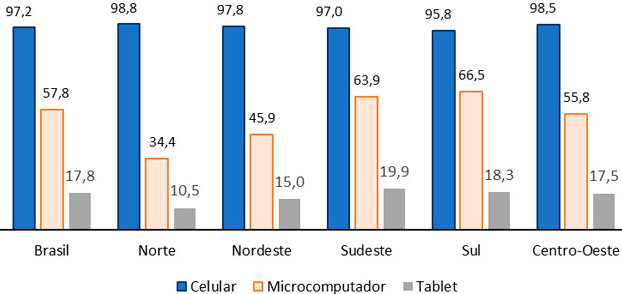
\includegraphics[width=0.6\linewidth]{Imagens/grafico} 	
	\legend{Fonte: \citeonline{agencia_ibge_noticias2018}}
 \end{figure}
 
  Ambientes urbanos são os espaços de produção e reprodução da vida social e onde as oportunidades de trabalho, educação, saúde, cultura, lazer e todas outras dimensões da vida cotidiana se concentram. O \citeonline[p.~19]{IBGEIBGE2011} define este termo como, "área legalmente definida como urbana, que se caracteriza por construções, arruamentos e intensa ocupação humana". Estes espaços vem  aumentando constantemente, como podemos ver na a Figura 2 abaixo. 
  \begin{figure}[H]
	\centering
 	\caption{Grau de urbanização, segundo as Grandes Regiões 1991/2010.} 
 	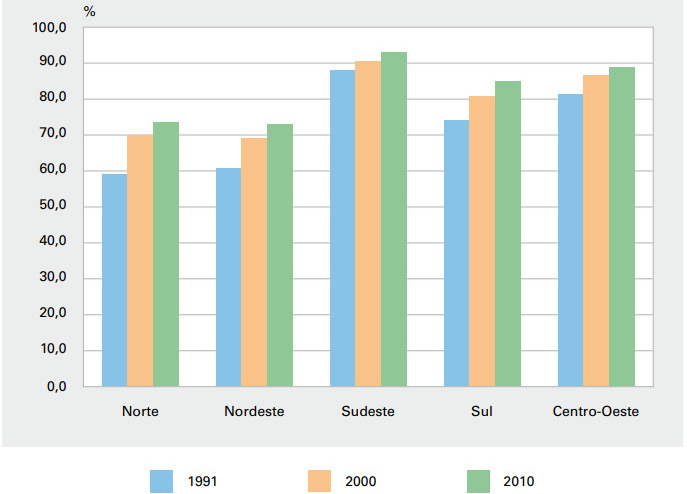
\includegraphics[width=0.6\linewidth]{Imagens/grafico2}		
	\legend{Fonte: \citeonline[p.~46]{IBGEIBGE2011} }
 \end{figure}  

 \citeonline[p.~7]{hyller_bandeira_dutra_cidadao_2018} realizou um levantamentos por meio de conversas informais com moradores, nas quais revelaram que são comuns as reivindicações da população em relação à resolução de problemas, utilizando canais de comunicação como a rádio local, o telefone da prefeitura, e mídias sociais como Facebook e WhatsApp. A variedade de meios de comunicação, embora conveniente, dificulta o gerenciamento e a gestão das informações fornecidas. 

 Desta maneira, uma aplicação de um sistema para dispositivos moveis como o Cidadão do Vale configura-se como uma alternativa via sistema informacional que possibilita a centralização, organização e georreferenciamento das informações. O emprego de um sistema mobile, associado aos conceitos de VGI, facilita a comunicação entre as pessoas e a gestão municipal ao proporcionar um veículo de comunicação com dados objetivos, disposição das informações de forma pública, com possibilidade, inclusive, de pesquisas sobre a situação do município.

\section*{Objetivo Geral} 
Facilitar o gerenciamento dos problemas na infraestrutura em Almenara – MG, por meio do desenvolvimento de um sistema Android baseado no Cidadão do Vale.
	
\section*{Objetivos Específicos}

\begin{flushleft}
	Como objetivos específicos pretende-se:
\end{flushleft}
\begin{itemize}
	\item Levantar requisitos do sistema web Cidadão do Vale;
	\item Desenvolver um aplicativo para dispositivos móveis com base no Cidadão do Vale;
	\item Atualizar o mapeamento dos problemas relacionados à infraestrutura urbana de Almenara;
	\item Alertar o poder público dos problemas na infraestrutura de Almenara – MG;
\end{itemize}

\section*{Justificativa}
A proposta justifica-se pela possibilidade de eliminação da necessidade de pesquisas de data fixa, onerosas ao poder público, já que o sistema web viabiliza o fluxo continuo de informações e, consequentemente, de resoluções. A manutenção de um canal público capaz de centralizar as informações sobre a infraestrutura urbana em ambiente WebGIS e a visualização integrada território almenarense poderá auxiliar no processo de tomada de decisões e facilitar o diálogo entre a população e a gestão pública. Tais iniciativas geram impactos positivos sobre o orçamento público e democratizam o acesso a informação sobre a gestão do espaço urbano, e reafirmam o compromisso do IFNMG previsto na Lei nº. 11.892/08 \citeonline{LILDS2008}, de “orientar sua oferta formativa em benefício da consolidação e fortalecimento dos arranjos produtivos, sociais e culturais locais, identificados com base no mapeamento das potencialidades de desenvolvimento socioeconômico e cultural no âmbito de atuação do Instituto Federal”.

\section*{Resultados Esperados}
Espera-se que o este trabalho continue suas contribuições para o desenvolvimento urbano de Almenara e estreite as relações entre o IFNMG e a gestão municipal. Além disso, a expectativa é de que o aplicativo desenvolvido aproxime a população municipal da gestão pública por meio de suas contribuições online medida. A transparência e o diálogo são meios fundamentais para o alcance da cidadania plena.

  %OK
%
%%%
%% Revisão Bibliográfica
%%%

\chapter{Referencial Teórico}

\section{Pessoas como Sensores Voluntários}
Para a compreensão da utilização de pessoas como sensores vê-se necessário o entendimento dos conceitos de User-generated content (UGC), World Wide Web 2.0 (WEB 2.0), Neogeografia, Inteligência Coletiva, e Volunteered Geographic Information (VGI), os quais serão apresentados a seguir. 

UGC (User-Genereted Content – Conteúdo Gerado pelo Usuário) segundo \cite{santos_avaliacao_2016}, se refere a ação dos usuários compartilharem suas experiências e com isso produzir um grande volume de informações. Um dos mais populares exemplos é a Wikipédia, uma plataforma colaborativa que contém mais de 1.000,000 artigos em português e 6,292 usuários ativos, este número vem crescendo constantemente \cite{Wikipedia2018}.

A WEB 2.0 representa uma maneira diferente de interagir com a internet, pois oferece maior autonomia para o usuário no sistema, na medida em que possibilita a criação de conteúdo e a avaliação daquilo que consome. \citeonline [p.~2]{Primo2007} afirma que Web 2.0 é a uma nova geração de serviços na rede, identificada  por suas diversas formas de produção contributiva e partilhamento de informações online. Plataformas como Twitter e Youtube, com centenas de milhões de usuários, tem se adaptando para melhor atender seu público por meio da implementação de recursos que facilitam tanto a criação quanto à visualização de conteúdo. 

O termo Neogeografia (nova geografia) para \citeonline[p.~228]{machado_os_2014} Machado (2014), é um fenômeno social que gira em torno do crescimento em massa dos mapas virtuais, e ao facilitamento de uso de tecnologias com ferramentas para posicionamento como o GPS.

Para \citeonline[p.~28]{Levy2007}, inteligência coletiva é "uma inteligência distribuída por toda parte, incessantemente valorizada, coordenada em tempo real, que resulta em uma mobilização efetiva das competências".

De acordo com \apudonline[p.~10]{Goodchild2007}{miranda_uma_2010}, VGI é uma expressão usado para definir a informações geográficas que são produzidas através de usuários, que funde elementos da Web 2.0, Inteligência Coletiva e Neogeografia e que atinge as necessidades da indústria, do governo e das comunidades de redes sociais. O conjunto de dados e as informações deles decorrentes são, por meio de plataformas de inteligência coletiva, avaliados, validados e consolidados pelos usuários, inclusive aqueles que geraram a informação.

\section{O Sistema WEB Cidadão do Vale}
Conforme exposto, a plataforma Cidadão do Vale foi implementada no município de Almenara-MG como alternativa a informação de problemas urbanos e de gestão municipal. O sistema Cidadão do Vale foi disponibilizado de forma pública sob o domínio \url{www.cidadaodovale.xyz}, em funcionamento completo que inclui a visualização e contribuição de dados do sistema. Na Figura 3 é apresentada a página inicial, onde se encontra as colaborações georreferenciadas cadastradas no sistema em 3 de agosto de 2018. A Figura 4 corresponde a tela de cadastro de usuário, e as Figuras 5 e 6 correspondem aos mapas de calor referentes às contribuições sobre limpeza urbana e vias públicas em 3 de agosto de 2018.

% PÁGINA INICIAL
\begin{figure}[H]
	\centering
	\caption{Página inicial da plataforma Cidadão do Vale.}
	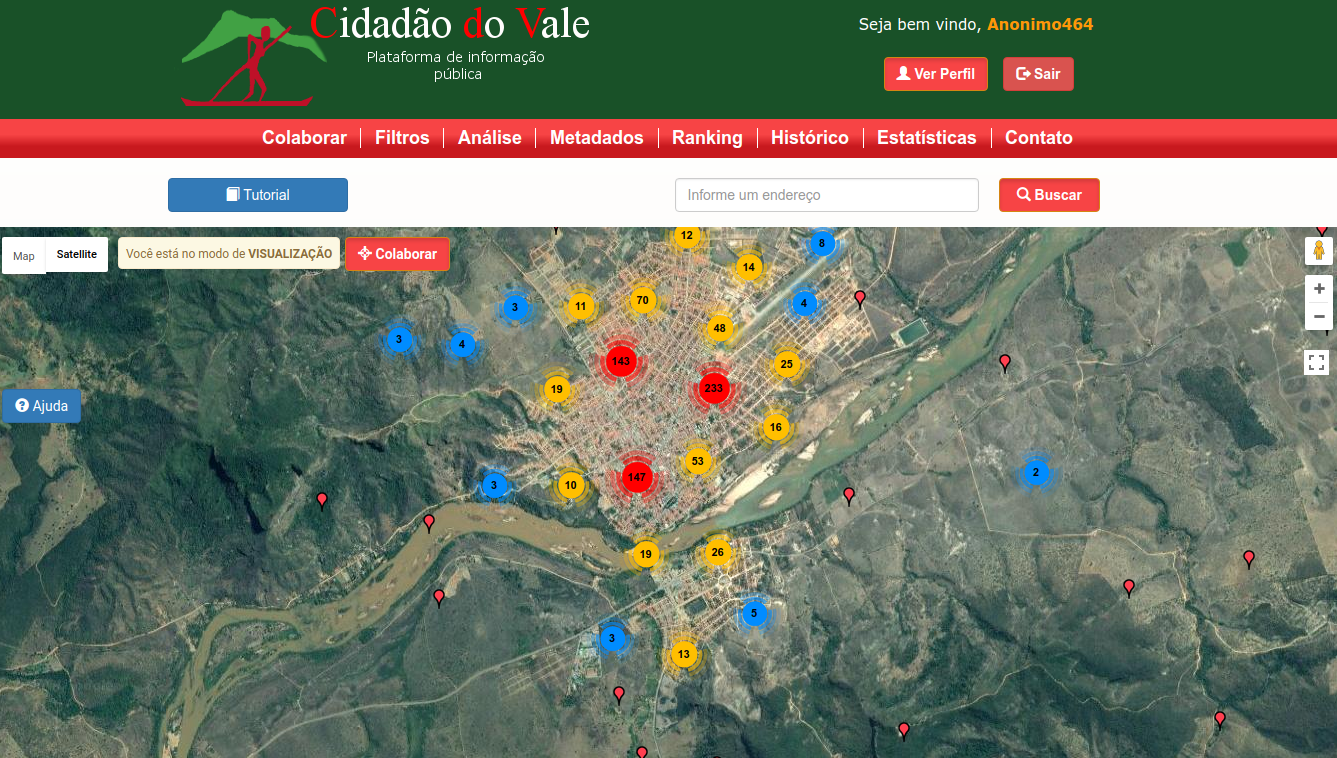
\includegraphics[width=0.6\linewidth]{Imagens/01}
	\legend{Fonte:\url{http://www.cidadaodovale.xyz/inicio.php}}
\end{figure}

% CADASTRO
\begin{figure}[H]
	\centering
	\caption{Página de cadastro do sistema Cidadão do Vale}	
	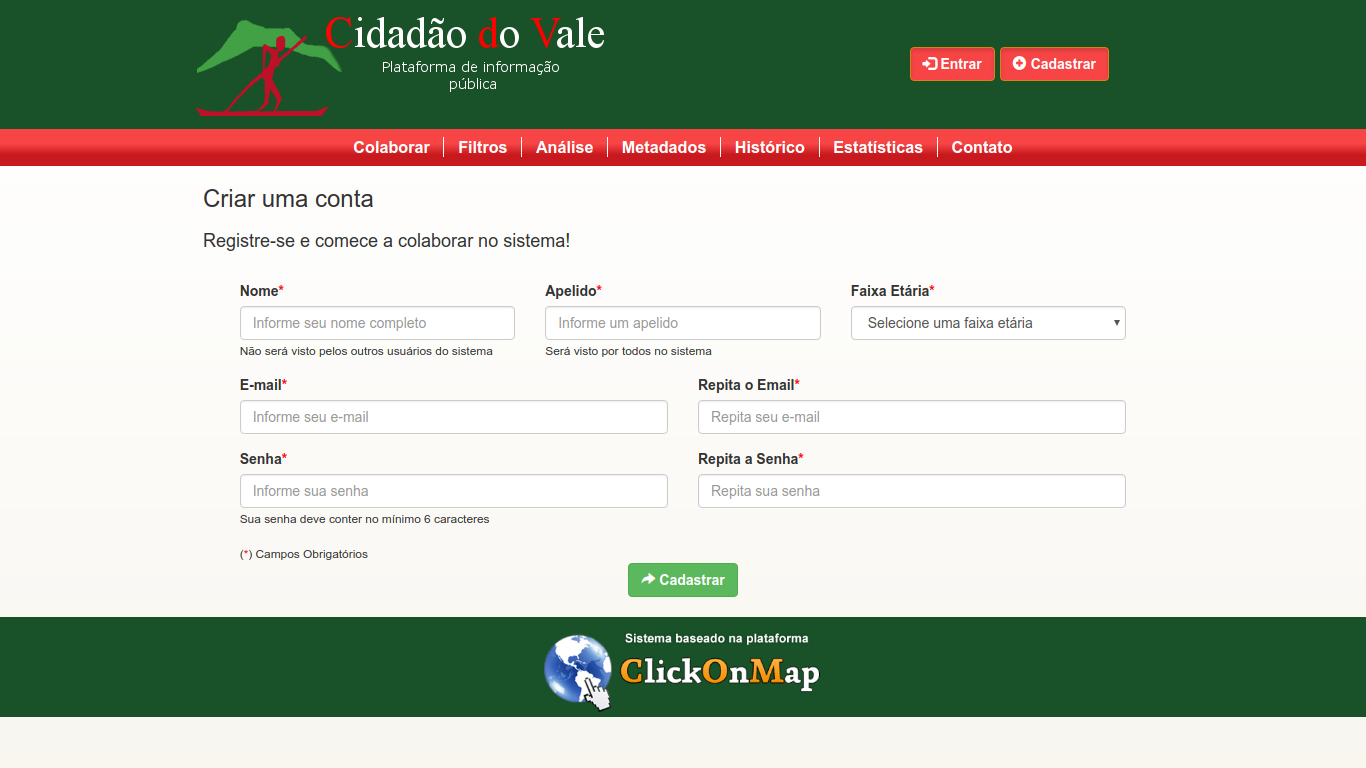
\includegraphics[width=0.6\linewidth]{Imagens/02}
	\legend{Fonte:\url{http://www.cidadaodovale.xyz/registro.php}}
\end{figure}

% LIMPEZA URBANA
\begin{figure}[H]
	\centering
	\caption{Densidade Kernel das contribuições sobre limpeza urbana.}
	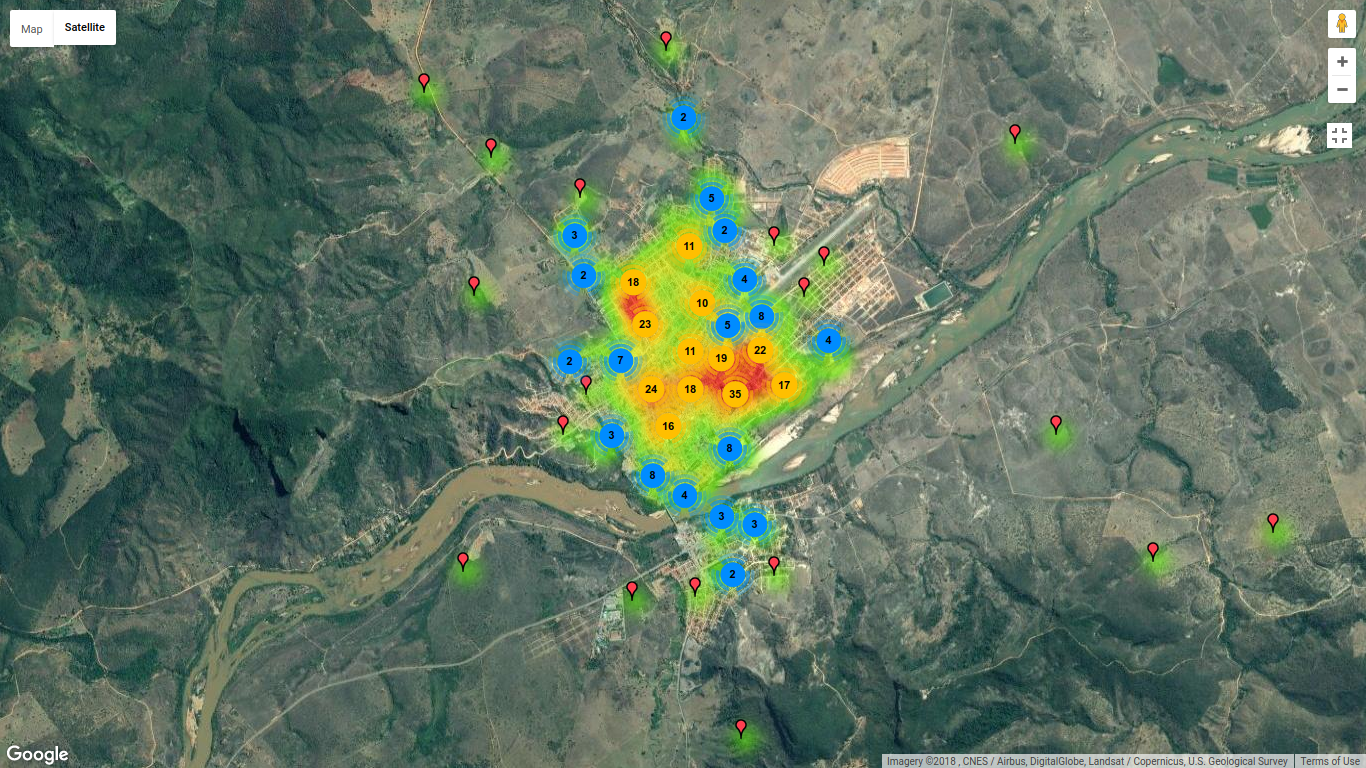
\includegraphics[width=0.6\linewidth]{Imagens/03}
	\legend{Fonte:\url{http://www.cidadaodovale.xyz/inicio.php}}
\end{figure}

% VIAS PÚBLICAS
\begin{figure}[H]
	\centering
	\caption{Densidade Kernel das contribuições sobre problemas nas vias públicas.}	
	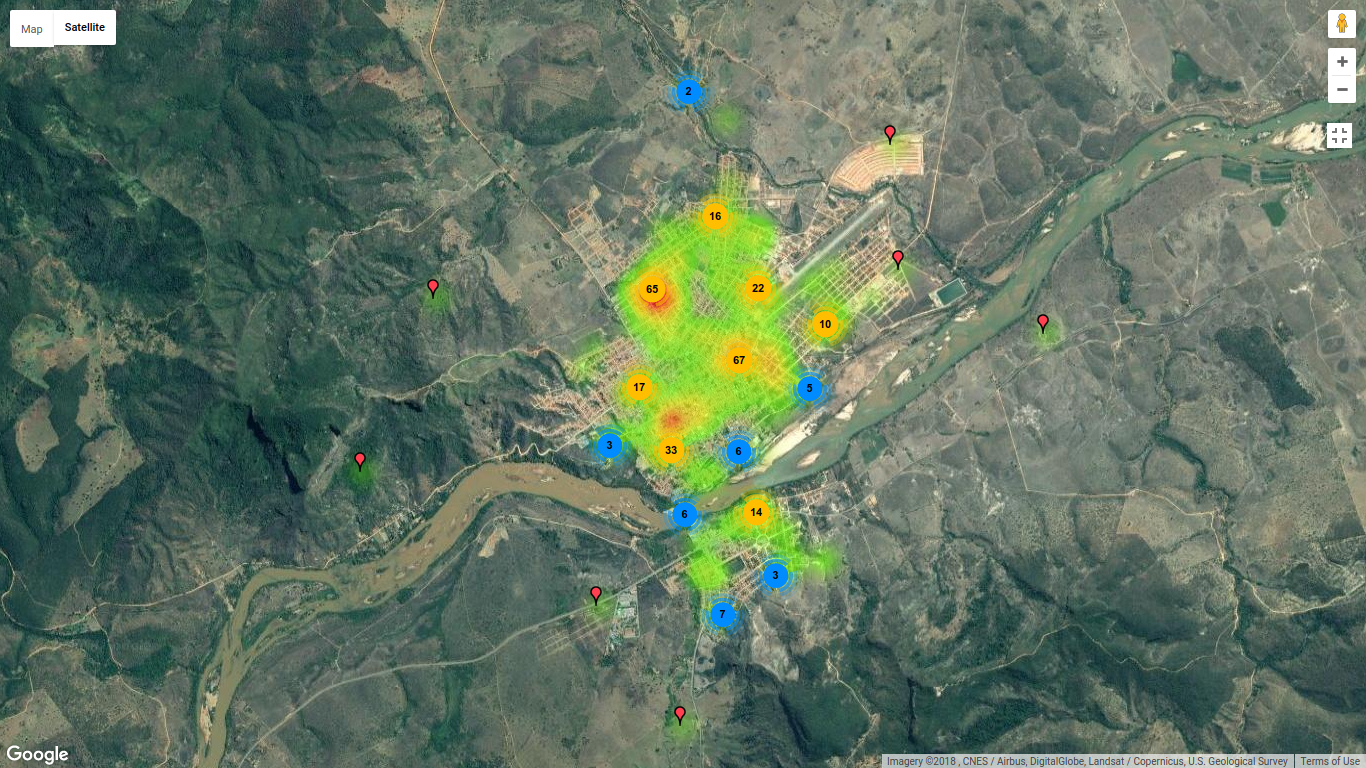
\includegraphics[width=0.6\linewidth]{Imagens/04}
	\legend{Fonte:\url{http://www.cidadaodovale.xyz/inicio.php}}
\end{figure}

\section{Cordova}
Conforme apresentado na documentação oficial \citeonline{the_apache_software_foundation_architectural_nodate} o Cordova é um framework de código aberto que permite a utilização de linguagens padrão da web para o desenvolvimento de aplicativos multiplataformas. Ele utiliza as linguagens padrão da web, HTML5\footnote{Hypertext Markup Language – linguagem de marcação de hipertexto.}, CSS3\footnote{Cascading Style Sheets – estilo de folha em cascata.}, e JavaScript.

\citeonline[p.~2]{lopes_sergio_aplicacao_2016} afirma que, o Cordova é responsável por criar uma "casca nativa" para o aplicativo, na qual gera uma janela de navegador, que faz comunicação entre as chamadas de código para chamadas nativas quando necessário. A Figura 7 mostra a arquitetura do Cordova, na qual utiliza de APIs para realizar a comunicação entre o sistema e o a web, possibilitando assim o acesso a funcionalidades de qualquer aparelho, como sensores, dados, status da rede etc . 

\begin{figure}[H]
	\centering
	\caption{Arquitetura do Cordova}	Cordova cria uma "casca nativa" para o aplicativo 
	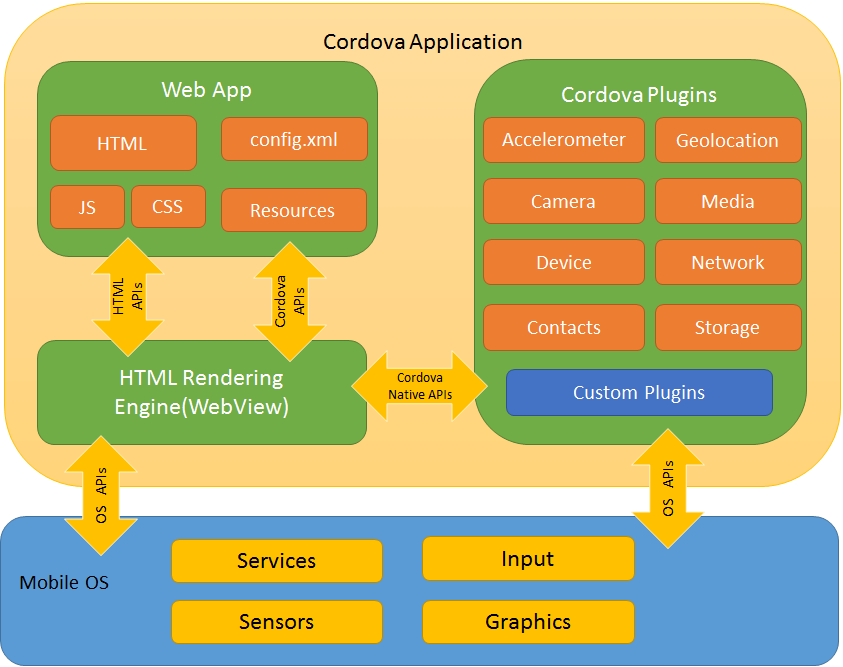
\includegraphics[width=0.6\linewidth]{Imagens/cordovaapparchitecture.png}
	\legend{Fonte:\url{https://cordova.apache.org/docs/en/latest/guide/overview/index.html}}
\end{figure}

\section{Firebase}
O Firebase é um sistema online desenvolvido pela Google do qual possui vários serviços, como banco de dados em tempo real, acesso offiline, aramaz
\citeonline{khawas_application_2018} afirma que o Firebase é uma plataforma online, que auxilia os de desenvolvedores a criarem aplicações de qualidade, ele trabalha com armazenamento NoSQL, no qual realiza os armazenamentos em formato JSON\footnote{JavaScript Object Notation - Objeto de notação JavaScript}, pela Google, que possui vários serviços para diversas plataformas. Segundo \citeonline{silva_junior_and_buregio_vanilson_2016} o Firebase possui uma sincronização em tempo real para Android, iOS e JavaScript, que possibilita o aplicativo esteja responsivo e funcionando offline.
 %OK
%
%%%
%% Metodologia da Pesquisa
%%%
% -----------------------------------
% METODOLOGIA DA PESQUISA
% -----------------------------------
\chaptertitlename{Metodologia}
\begin{flushleft}
	A metodologia de desenvolvimento deste trabalho consistiu em cinco etapas:
\end{flushleft}

\begin{enumerate}
		\item Compreensão da estrutura da plataforma web;
		\item Elaboração de um protótipo de aplicativo para aparelhos móveis adequado às características da plataforma;
		\item Definição dos pré-requisitos para viabilizar a conexão entre a plataforma web e o aplicativo;
		\item Implementação do aplicativo para dispositivos móveis na plataforma livre Android;
		\item Alimentação da plataforma;
\end{enumerate}

A principio foi realizado uma análise da plataforma Cidadão do Vale, para compreensão do funcionamento e estruturação do sistema. Foi considerado que a implementação tem sido realizada de maneira coletiva e colaborativa, e que se trata de um sistema já em funcionamento, a familiarização com a interface e programação da plataforma foi uma etapa crucial para o desenvolvimento.

A segunda fase, elaborou-se um protótipo do aplicativo no qual buscou replicar os elementos da interface da plataforma web de maneira intuitiva e amigável.

No terceiro momento, foi estudado os pré-requisitos para viabilizar a conexão entre a plataforma web e o aplicativo. Neste caso, foram avaliadas as características e vantagens de se desenvolver aplicativos dos tipos nativos, Web Apps, ou híbridos. Segundo informações de \citeonline{madureira_aplicativo_2017}, em síntese, eles se diferenciam pela linguagem utilizada e pelo tráfego de dados utilizados. Os nativos são programados em linguagem exclusiva para dispositivos móveis, são mais rápidos e confiáveis. Os Web Apps não são aplicativos reais, mas sim sites desenvolvidos para dispositivos móveis. As vantagens são o funcionamento em qualquer sistema operacional e o fato de não ocupar espaço na memória dos aparelhos. A desvantagem é que requer conexão com a internet para funcionamento. Por fim, os aplicativos híbridos são aqueles em que mesclam características dos nativos e Web Apps. Sua elaboração é mais simples, entretanto, requer internet para o funcionamento e não possui a mesma velocidade de resposta que um nativo. 

Após análizar todas as possibilidade, optou-se por desenvolver o aplicativo de forma hibrida, utilizando o framework Cordova. A decisão foi tomada com base nas necessidades de realizar contribuições sem internet, ter uma boa integração com a página web e que usa-se uma linguagem padrão que converse com o site, além destes pontos o Cordova possui uma boa documentação, é de código aberto, oque da uma maior liberdade para adaptação e desenvolve aplicativos multiplataformas.

Durante todo o desenvolvimento foram realizados testes, tais testes permitiram aferir a qualidade do seu funcionamento, incluindo a velocidade e capacidade de transmissão de dados, intuitibilidade, manuseio, erros e travamentos. Está fase foi primordial para o desenvolvimento, e foi realizada constantemente durante o processo.

Por fim foi realizado a alimentação da plataforma com informações atuais sobre o município. O aplicativo será divulgado e disponibilizado para o público, para coleta e análise das informações atualizadas.

\chapter{Resultados obtidos} %OK
%
%%%
%% Cronograma das atividades de pesquisa
%%%
\include{Cronograma/cronogramadapesquisa} %OK
%
%%%
%% Conclusão
%%%

% ---------
% Conclusão
% ---------
\chapter*{CONSIDERAÇÕES FINAIS}
\addcontentsline{toc}{chapter}{CONSIDERAÇÕES FINAIS}
\label{cap:Conclusao}
Realizou-se o desenvolvimento do aplicativo cidadão do vale em versão beta devido a complexidade de integrar os dados da plataforma Firebase usada para salvar informações do aplicativo com o banco de dados MySQL, usado para  salvar as contribuições feitas pela plataforma web.
A versão beta do aplicativo desempenha a função de informar problemas urbanos em tempo real com integração ao GPS, isso representa um avanço na usabilidade da plataforma web, na qual necessita que o endereço seja digitado, podendo gerar erros. 
Os resultados apresentados por esse trabalho são iniciais, abrindo possibilidade para trabalhos futuros de desenvolver os módulos de deletar, atualizar e visualizar colaborações.


 %OK

% ----------------------------------------------------------
% Referências bibliográficas
% ----------------------------------------------------------

\renewcommand{\bibname}{REFER\^ENCIAS}

\bibliography{Bibliografia/Referencias}

\end{document}
